\documentclass{article}

\usepackage{tikz}
\usepackage[margin=1in]{geometry}

\begin{document}

\begin{figure}[h]
\centering
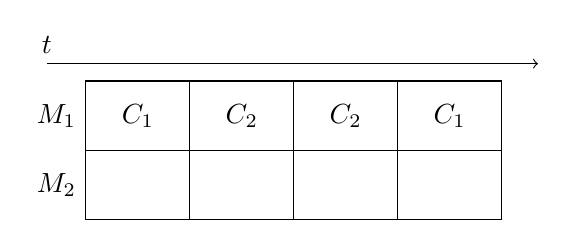
\begin{tikzpicture}[scale=1.1]

% Grid dimensions
\def\w{1.2}
\def\h{0.8}

% Draw outer rectangle and internal grid lines
\draw (0,0) rectangle (4*\w,2*\h);

\foreach \i in {1,2,3} {
    \draw (\i*\w,0) -- (\i*\w,2*\h);
}

\draw (0,\h) -- (4*\w,\h);

% Completion time labels
\node at (0.5*\w,1.5*\h) {$C_1$};
\node at (1.5*\w,1.5*\h) {$C_2$};
\node at (2.5*\w,1.5*\h) {$C_2$};
\node at (3.5*\w,1.5*\h) {$C_1$};

% Machine labels
\node[left] at (0,1.5*\h) {$M_1$};
\node[left] at (0,0.5*\h) {$M_2$};

% Time axis
\draw[->] (-0.45,2.25*\h) -- (4.35*\w,2.25*\h);
\node[above] at (-0.45,2.25*\h) {$t$};

\end{tikzpicture}
\caption{Illustration for a scheduling proof.}
\end{figure}

\end{document}